\documentclass[11pt]{amsbook}

\usepackage{../HBSuerDemir}

\begin{document}

% ++++++++++++++++++++++++++++++++++++++
\hPage{b2p2/318}
% ++++++++++++++++++++++++++++++++++++++
\begin{hSolution}
	\begin{minipage}{0.6\textwidth}
		\begin{align*}
			r_\lambda : & F(x, y, \lambda) = (x - \lambda)^2 + y^2 - r^2 = 0    \\
			            & F_\lambda = -2 (x - \lambda) = 0 \implies x = \lambda
		\end{align*}

		Then
		\[
			(x - \lambda)^2 + y^2 - r^2 = 0, x = \lambda
		\]

		are the parametric equation of the envelope.
	\end{minipage}
	\begin{minipage}{0.4\textwidth}
		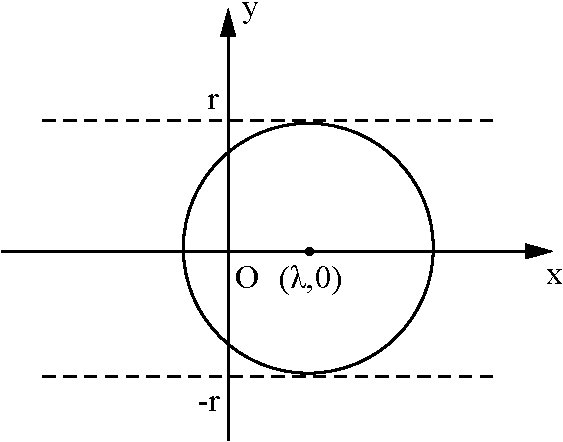
\includegraphics[width=1\textwidth, keepaspectratio]{images/b2p2-318-fig01}
	\end{minipage}\\

	Then eliminating $\lambda$, one gets
	\[
		y^2 - r^2 = 0 \implies y = \pm r
	\]
	showing that the envelope consists of two lines parallel to x-axis.
	This envelope is the locus of heighest and lowest points (characteristic points)
	of the circles.
\end{hSolution}

\begin{exmp}
	Find the envelope of the family
	\[
		r_\lambda: F(x, y, \lambda) = 2 (x - \lambda)^3 - 3 (y - \lambda)^2 = 0
	\]

	\begin{hSolution}
		The curve $r_\lambda$ is related to $r_0: 2x^3 - 3y^2 = 0$
		by the translation $(\lambda, \lambda)$, and $r_0$ admits a cusp\footnotemark
		at the origin.\\

		\begin{minipage}{0.69\textwidth}
			Since
			\[
				F_\lambda(x, y, \lambda) = -6 (x - \lambda)^2 + 6 (y - \lambda) = 0
			\]
			we have the envelope:
			\[
				e: 2 (x - \lambda)^3 - 3 (y - \lambda)^2 = 0,
				(x - \lambda)^2 - (y - \lambda) = 0
			\]

			To eliminate $\lambda$, setting $y - \lambda = (x - \lambda)^2$
			in the first, we have
			\[
				2 (x - \lambda)^3 - 3 (x - \lambda)^4 = 0
				\implies
				(x - \lambda)^3 (2 - 3 (x - \lambda)) = 0
			\]

			\begin{multicols}{2}
				\begin{hEnumerateRoman}
					\item
					\begin{center}
						$x - \lambda = 0$
					\end{center}

					\item
					\begin{center}
						$x - \lambda = \frac{2}{3}$
					\end{center}
				\end{hEnumerateRoman}
			\end{multicols}
		\end{minipage}
		\begin{minipage}{0.31\textwidth}
			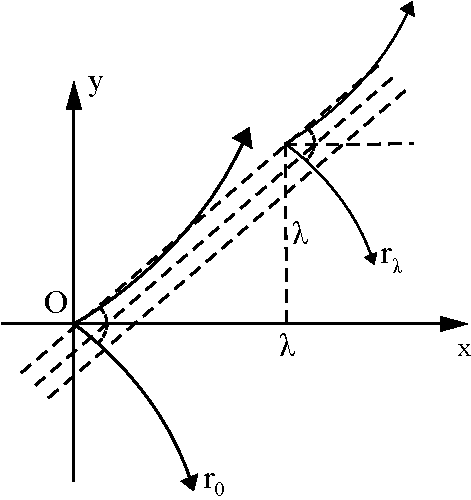
\includegraphics[width=1\textwidth, keepaspectratio]{images/b2p2-318-fig02}
		\end{minipage}
	\end{hSolution}

	\footnotetext{A \textit{cusp} is a double point at which two tangent lines
		are coincident.
		\begin{multicols}{3}
			\begin{center}
				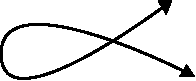
\includegraphics[width=0.13\textwidth, keepaspectratio]{images/b2p2-318-fig03}\\
				\vspace*{\fill} % Fill the vertical space above so that our texts are vertically aligned on bottom
				A double point
			\end{center}

			\begin{center}
				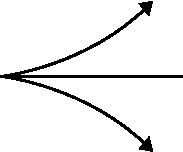
\includegraphics[width=0.13\textwidth, keepaspectratio]{images/b2p2-318-fig04}\\
				\vspace*{\fill}
				A cusp of the first kind
			\end{center}

			\begin{center}
				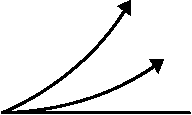
\includegraphics[width=0.13\textwidth, keepaspectratio]{images/b2p2-318-fig05}\\
				\vspace*{\fill}
				A cusp of the second kind
			\end{center}
		\end{multicols}}
\end{exmp}

\end{document}
